\documentclass[10pt,usenames,dvipsnames,svgnames,table]{beamer}
\usetheme{Warsaw}

\usepackage[english]{babel}
\usepackage[latin1]{inputenc}
\usepackage{amssymb}
\usepackage{graphicx}
\usepackage{epstopdf}
\graphicspath{ {./images/} }
\allowdisplaybreaks
\usepackage{tikz}
\usepackage{algorithm,algpseudocode}
\setbeamertemplate{bibliography item}[text] %remove the icon
\setbeamertemplate{frametitle continuation}{}

\title[Optimal Location of Car Wreck Adjusters]
      {Optimal Location of Car Wreck Adjusters}
\subtitle{DOS Team}
\author[Luis Maltos, Roger R\'ios, Angelica Salazar, M. Gpe. Villarreal]{
  L. A. Maltos-Ortega \inst{1},
  R. Z. R\'ios-Mercado \inst{1},
  M. A. Salazar-Aguilar \inst{1}
  \and M. G. Villareal Marroquin \inst{2}}

\institute[PISIS]{
  \inst{1} Graduate Program in Systems Engineering \\
  FIME / UANL \and
  \inst{2} CIMAT Unidad Monterrey
}

\date[Feb 2016]{February 2016}

\logo{
  \makebox[0.95\paperwidht]{
    \hspace{-60pt}
    
\includegraphics[width=1.5cm,keepaspectratio]{pisis_logo}
  }
}

\AtBeginSubsection{
  \frame{\frametitle{Table of Contents}
    \tableofcontents[currentsubsection]}
}

\begin{document}
\begin{frame}
  \titlepage
\end{frame}

\begin{frame}{Contents}
  \tableofcontents
\end{frame}

%%% Introduction %%%

%En ella se deben exponer brevemente pero con absoluta claridad, 
% la novedad y actualidad del tema,
% el objeto de la investigacion,
% sus objetivos,
% la hipotesis de trabajo,
% el fundamento metodologico y
% los metodos utilizados para realizar el trabajo de investigacion.
%Es decir, que la introduccion es
% la fundamentacion cientifica de la tesis en forma resumida.

\section{Introduction}
\begin{frame}
  The aim of this work
  is to support decision making
  regarding the location and redeployment
  of insurance agents to attend car wrecks.

  The idea is to
  develop models and methods for 
  (a) improving the service 
  offered by insurance agents, 
  helping them
  arrive to the accident sites sooner,
  and 
  (b) determining the number of adjusters
  required to perform the service
  within the desired standards.

\end{frame}

\subsection{Problem}
\frame{
  The main goal is to
  determine the optimal bases (locations) 
  for placing the insurance company adjusters, 
  so as to minimize
  the average or maximum response time
  from customer calls
  when accidents occur.
  \begin{center}
    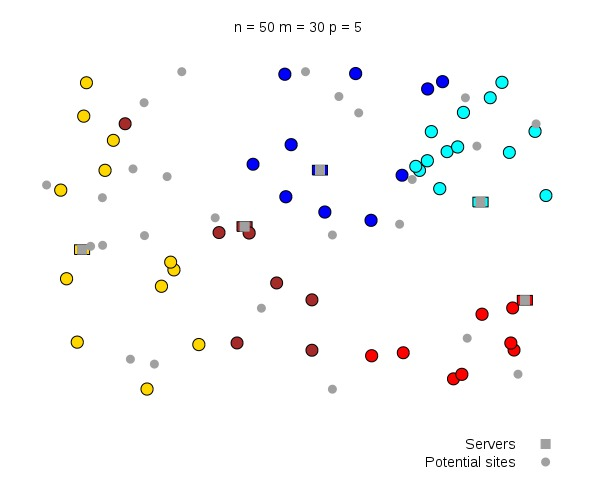
\includegraphics[scale=0.35]{SQpM_problem}
  \end{center}
}

\subsection{Motivation}
\begin{frame}
  When a car accident occurs,
  traffic congestion starts to pile up.
  This is because
  customers are not allowed
  to move their vehicles
  until the adjuster arrives.  
  The adjuster must record and determine
  the causes of the accident, 
  in order to
  move the car from the accident area
  and restore the flow.
  \begin{center}
    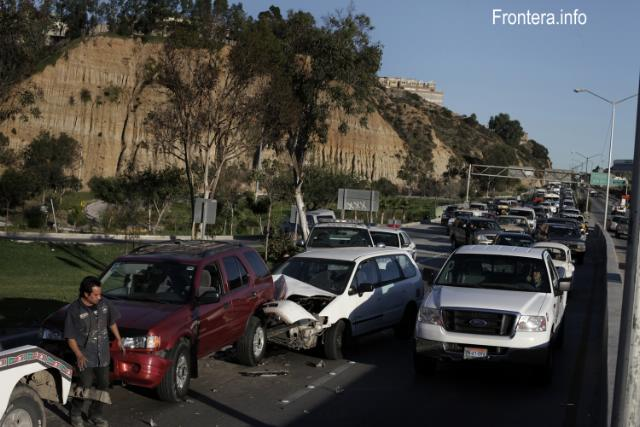
\includegraphics[scale=0.25]{389200-G}
  \end{center}
\end{frame}


\section{Heuristics}
\subsection{Evaluation}
\begin{frame}
  The objective function to considered is one that estimates the average time of arrival of the adjusters.
  \begin{equation}
    \sum_{i=1}^{p}{\sum_{k=1}^p{\sum_{j|a_{jk}=i}{f_{ij}\tau_{ij}}}}
  \end{equation}
  for evaluation, values of $f_{ij}$ are required. 
\end{frame}

% The Stochastic Queue p-Median Problem
% O. Berman, R.C. Larson, C. Parkan 
% 1987
\subsection{Improvement}
\begin{frame}
  This problem is presented by Berman et al. \cite{berman1987stochastic}

  \begin{itemize}
  \item $G(N,L)$ the transportation network
  \item $N$ the set of demand centers,
    with $|N| = n$
  \item $L$ the set of all transportation arteries,
    the links
  \item $h_j$ the fraction of service calls
    associated with each node $j$
  \item $d(X,Y)$ is the shortest path between any two points $X,Y \in G$
  \item $p$ number of response units
  \item $\bar{X}$ the home locations of the service units while available
  \item $\lambda$ mean rate per unit of time
    within service calls are generated in Poisson manner
  \end{itemize}
\end{frame}

\begin{frame}
  Given the arrival of a call for service,
  exactly one of the servers is dispatched to it
  assuming that at least one server is available.

  The service time for any service unit \textit{i}
  is the sum of two components:
  \begin{itemize}
  \item The non-travel time component,
    which is the sum of
    on-scene and off-scene service time.
  \item Travel time component,
    which is the sum of travel time
    to the location of the call
    and travel time back to the home location.
  \end{itemize}
\end{frame}

\begin{frame}
  The mean service time 
  for a service unit located at $\bar{X}^i$ 
  is denoted $S(\bar{X}^i)$,
  \begin{equation}
    S(\bar{X}^i) =
    \sum_{j = 1}^{n} {
      h_j^i\left(
      \bar{W}_{ij}
      +\frac{{\beta}_i}{v_i}d(\bar{X}^i,j)
      \right)
    } \; i=1,\ldots,p
  \end{equation}
  \begin{itemize}
  \item $\bar{W}_{ij}$ is the mean
    of the \textbf{non-travel time} component $W_{ij}$
  \item $v_i$ is the \textbf{travel speed} of unit \textit{i}
    to the scene of the call
    which is assumed constant
  \item $\beta_i$ is a constant
    that allows different travel speeds
    to and from the scene of the call
  \item $h_j^i$ is the probability that server \textit{i} 
    is dispatched to node \textit{j}
    given that server \textit{i}
    is dispatched to a call for service.
  \end{itemize}
\end{frame}

\begin{frame}
  Whenever a call for service arrives 
  while at least one of the servers
  is free at its home location,
  the closest available server to the call
  will be dispatched.
  Calls that find
  all servers busy
  enter a queue.
  The queue discipline is assumed to be
  First-Come-First-Served.
  The expected response time
  to a random call
  denoted by $\bar{T}_R(X)$
  is the sum of two components
  \begin{equation*}
    \bar{T}_R(\bar{X}) = \bar{W}_q(\bar{X})+\bar{t}(\bar{X})
  \end{equation*}
  \begin{itemize}
  \item $\bar{W}_q(\bar{X})$ is the expected \textbf{waiting time} in the queue
  \item $\bar{t}(\bar{X})$ is the expected \textbf{travel time} to the call.
  \end{itemize}
  The objective is to find
  a set of \textit{p} locations $\bar{X}^*$
  on the network
  such that
  \begin{equation*}
    \bar{T}_R(\bar{X}^*) \leq \bar{T}_R(\bar{X}) \; \forall \bar{X} \in G
  \end{equation*}
  $\bar{X}^*$ is called \textbf{the stochastic queue p-median}.
\end{frame}

\newcounter{iteration}
\forloop{iteration}{1}{\value{iteration} < 5} {
  \frame{
    \begin{figure}[h!]
      \begin{center}
        \includegraphics[scale=0.45]{SQM_Heuristic_\arabic{iteration}}
        \caption{m = n = 30, p = 5, iteration = \arabic{iteration}} 
      \end{center}
    \end{figure}
  }
}


\subsection{Path Relinking}
\begin{frame}{}{}
  \begin{algorithm}[H]
    \caption{Path Relinking Algorithm}
    \label{algPR}
    \begin{algorithmic}
      \State \textbf{Input:} $X,Y$ SQpMSols
      \State PathRelinkingSols = EmptyList()
      \State match = MatchingFunction(X,Y)
      \State order = ProcessingOrderFunction(X,pm,Y)
      \For {$i=0$ \To $p$}
      \If{X.location[order[i]] != Y.location[match[order[i]]]}
      \State Z = X.clone()
      \State Z.location[order[i]] = Y.location[match[order[i]]]
      \State PathRelinkingSols.insert(Z)
      \State X = Z
      \EndIf
      \EndFor
    \end{algorithmic}
  \end{algorithm}
\end{frame}


%%% Future Work %%

%Things to not do in your conclusion:

%   Introduce new information.
% The conclusion is for wrapping up everything you hacve done.
% It's not a place to say “oh yeah,
% and we also got result y.”
% All results should be first presented and detailed in the result section.
% Think of the conclusion as a place to reflect on what you have
% already said earlier in the paper.
%   Directly re-quote anything you’ve already written.
% I’ve seen conclusions that are almost identical
% to the abstract or a collection of sentences from throughout the paper.
% As a reader, it makes me think the author was lazy
% and could not be bothered to actually summarize their results for the paper.
% Take the time to write a proper conclusion
% so that the reader walks away with good thoughts about your work.
%   Write a conclusion longer than your introduction.
% A conclusion should be short, and to the point.
% You’ll rarely see them over 3 paragraphs,
% and three is often long.
% A lot of the time they are usually only one or two.
% Think about a conclusion as a chance to see
% how concisely you can summarize your entire research project.
% It’s your “30 second” research spiel.

\section{Future Work}
\subsection{Future Work}
\begin{frame}{Future Work}
  \begin{itemize}
  \item \textst{Design and implement heuristic methods to perform a local search}
  \item \textst{Develop a simulator to evaluate the quality of the solutions}
  \item Running pending tests
  \item Generate instances from real data
  \end{itemize}
\end{frame}


\subsection{Acknowledgements}
\begin{frame}{Acknowledgements}
\begin{itemize}
\item CONACYT (Graduate Fellowship)
\item CONACYT (grant 2011-1-166397)
\item UANL
\item FIME
\end{itemize}

\end{frame}


%%% References %%%
\subsection{References}
\begin{frame}[allowframebreaks]
  %\setbeamertemplate{bibliography item}{\insertbiblabel}
  \frametitle{References}
  {\scriptsize
    \bibliographystyle{abbrv}
    \bibliography{references}
  }
\end{frame}
\end{document}
